%   Copyright 2016 Emilio Rojas
%
%   Licensed under the Apache License, Version 2.0 (the "License");
%   you may not use this file except in compliance with the License.
%   You may obtain a copy of the License at
%
%       http://www.apache.org/licenses/LICENSE-2.0
%
%   Unless required by applicable law or agreed to in writing, software
%   distributed under the License is distributed on an "AS IS" BASIS,
%   WITHOUT WARRANTIES OR CONDITIONS OF ANY KIND, either express or implied.
%   See the License for the specific language governing permissions and
%   limitations under the License.

\documentclass[12pt]{article}

%   Copyright 2016 Emilio Rojas
%
%   Licensed under the Apache License, Version 2.0 (the "License");
%   you may not use this file except in compliance with the License.
%   You may obtain a copy of the License at
%
%       http://www.apache.org/licenses/LICENSE-2.0
%
%   Unless required by applicable law or agreed to in writing, software
%   distributed under the License is distributed on an "AS IS" BASIS,
%   WITHOUT WARRANTIES OR CONDITIONS OF ANY KIND, either express or implied.
%   See the License for the specific language governing permissions and
%   limitations under the License.

% Estos son los paquetes que se utilizan en los diferentes documentos del
% repositorio.
% Se mantienen ordenados primeramente por la cantidad de caractéres del nombre
% del paquete y luego por el orden alfabético. La excepción a esto es el  último
% grupo de paquetes, el cual tiene configuraciones.

\usepackage{url}

\usepackage{cite}
\usepackage{tikz}

\usepackage{color}
\usepackage{float}

\usepackage{amsmath}
\usepackage{apacite}
\usepackage{gensymb}
\usepackage{siunitx}

\usepackage{amsfonts}
\usepackage{etoolbox}
\usepackage{fancyhdr}
\usepackage{graphicx}
\usepackage{geometry}
\usepackage{hyperref}
\usepackage{multirow}
\usepackage{pdfpages}
\usepackage{pgfplots}
\usepackage{setspace}
\usepackage{textcomp}

\usepackage{circuitikz}

\usepackage[T1]{fontenc}
\usepackage[spanish]{babel}
\usepackage[utf8]{inputenc}

%   Copyright 2016 Emilio Rojas
%
%   Licensed under the Apache License, Version 2.0 (the "License");
%   you may not use this file except in compliance with the License.
%   You may obtain a copy of the License at
%
%       http://www.apache.org/licenses/LICENSE-2.0
%
%   Unless required by applicable law or agreed to in writing, software
%   distributed under the License is distributed on an "AS IS" BASIS,
%   WITHOUT WARRANTIES OR CONDITIONS OF ANY KIND, either express or implied.
%   See the License for the specific language governing permissions and
%   limitations under the License.

% allows to use < and > on tikz pictures when babel set to spanish
% http://tex.stackexchange.com/questions/166772/problem-with-babel-and-tikz-using-draw

\usetikzlibrary{babel}
\usetikzlibrary{positioning}
\usetikzlibrary{quotes,angles}

\pgfplotsset{compat=1.13}

\setlength{\columnsep}{1cm}

\patchcmd{\chapter}{\thispagestyle{plain}}{\thispagestyle{fancy}}{}{}

\geometry{
a4paper,
left=25.4mm,
right=25.4mm,
top=25.4mm,
bottom=25.4mm,
heightrounded,
}


% DIODO ZENER
\makeatletter
\pgfcircdeclarebipole{}{
  \ctikzvalof{bipoles/diode/height}
}{fullzzdiode}{
  \ctikzvalof{bipoles/diode/height}
}{
  \ctikzvalof{bipoles/diode/width}
}{

  \pgfsetlinewidth{\pgfkeysvalueof{/tikz/circuitikz/bipoles/thickness}\pgfstartlinewidth}

  \pgfscope
    \pgftransformxshift{\pgf@circ@res@left}
    \pgfpathmoveto{\pgfpoint{\pgf@circ@res@right-\pgf@circ@res@left}{0pt}}
    \pgfpathlineto{\pgfpoint{0pt}{\pgf@circ@res@up}}
    \pgfpathlineto{\pgfpoint{0pt}{\pgf@circ@res@down}}
    \pgfpathlineto{\pgfpoint{\pgf@circ@res@right-\pgf@circ@res@left}{0pt}}
    \pgfusepath{draw,fill}
    \pgfpathmoveto{
      \pgfpoint{
        \pgf@circ@res@right-1.8\pgf@circ@res@left
      }{
        \pgf@circ@res@down-0.5\pgf@circ@res@up
      }
    }
    \pgfpathlineto{
      \pgfpoint{
        \pgf@circ@res@right-\pgf@circ@res@left
      }{
        \pgf@circ@res@down
      }
    }
    \pgfpathlineto{
      \pgfpoint{
        \pgf@circ@res@right-\pgf@circ@res@left
      }{
        \pgf@circ@res@up
      }
    }
    \pgfpathlineto{
      \pgfpoint{
        \pgf@circ@res@right-0.2\pgf@circ@res@left
      }{
        \pgf@circ@res@up-0.5\pgf@circ@res@down
      }
    }
    \pgfusepath{draw}
  \endpgfscope
}
\def\pgf@circ@fullzzdiode@path#1{\pgf@circ@bipole@path{fullzzdiode}{#1}}
\tikzset{full Zzener diode/.style = {\circuitikzbasekey, /tikz/to path=\pgf@circ@fullzzdiode@path}}
\tikzset{zzD*/.style = {full Zzener diode}}
\makeatother

\sisetup{output-exponent-marker=\textsc{e}}
\setlength{\jot}{10pt}

\pagestyle{fancy}
\fancyhf{}
\lhead{Electrónica I}
\rfoot{\thepage}
\setlength{\headheight}{20pt}

\author{Emilio Javier Rojas Álvarez}

%   Copyright 2016 Emilio Rojas
%
%   Licensed under the Apache License, Version 2.0 (the "License");
%   you may not use this file except in compliance with the License.
%   You may obtain a copy of the License at
%
%       http://www.apache.org/licenses/LICENSE-2.0
%
%   Unless required by applicable law or agreed to in writing, software
%   distributed under the License is distributed on an "AS IS" BASIS,
%   WITHOUT WARRANTIES OR CONDITIONS OF ANY KIND, either express or implied.
%   See the License for the specific language governing permissions and
%   limitations under the License.

\definecolor{azulOscuro}{rgb}{0.02,0.02,0.7}
\definecolor{grisClaro}{rgb}{0.9,0.9,0.9}
\definecolor{grisOscuro}{rgb}{0.2,0.2,0.2}
\definecolor{commentColor}{rgb}{0.5,0.7,0.5}
\definecolor{negro}{rgb}{0,0,0}

%   Copyright 2016 Emilio Rojas
%
%   Licensed under the Apache License, Version 2.0 (the "License");
%   you may not use this file except in compliance with the License.
%   You may obtain a copy of the License at
%
%       http://www.apache.org/licenses/LICENSE-2.0
%
%   Unless required by applicable law or agreed to in writing, software
%   distributed under the License is distributed on an "AS IS" BASIS,
%   WITHOUT WARRANTIES OR CONDITIONS OF ANY KIND, either express or implied.
%   See the License for the specific language governing permissions and
%   limitations under the License.

% Unnumbered section added to toc
% 1: The section's name.
\newcommand{\usection}[1]
{
  \section*{#1}
  \addcontentsline{toc}{section}{#1}
}

% Unnumbered subsection added to toc
% 1: The subsection's name.
\newcommand{\usubsection}[1]
{
  \subsection*{#1}
  \addcontentsline{toc}{subsection}{#1}
}

% Unnumbered subsubsection added to toc
% 1: The subsubsection's name.
\newcommand{\usubsubsection}[1]
{
  \subsubsection*{#1}
  \addcontentsline{toc}{subsubsection}{#1}
}

% Circuitikz equal
\newcommand*{\equal}{=}

% Adds a title page to the document
% 1: The document's name
% 2: The document's date
\newcommand{\portada}[2]
{
\begin{titlepage}
  \vspace*{\fill}
  \begin{center}

    \textsc{\Large Universidad de Costa Rica}\\
    [0.25in]

    \textsc{\Large Escuela de Ingienería Eléctrica}\\
    [0.55in]

    \textsc{\Large Electrónica I - IE0313}\\
    [0.25in]

    \textsc{\huge \bfseries {#1}}\\
    [0.5in]

    \textsc{\large Emilio Javier Rojas Álvarez}\\
    \textsc{\large B15680}\\
    [0.5in]

    \textsc{\large {#2}}

  \end{center}
  \vspace*{\fill}
\end{titlepage}
}


\begin{document}

\pagenumbering{gobble}
\portada{Tarea \#1}{6 de Octubre, 2016}

\pagenumbering{arabic}

\section{}

Para el circuito mostrado, obtenga

\begin{itemize}
  \item El valor DC de la corriente y el voltaje del diodo(punto de
  operación).
  \item El valor de $V_o$ en función de $V_i$.
\end{itemize}

\begin{figure}[H]
  \begin{center}
    \begin{circuitikz}

      \draw (0,0)
      to [sV, l=$v_i$] (0, 6)
      to [R, l=$100\Omega$] (2.5, 6)
      to [C, l=$C \to \infty$] (5, 6)
      to [D*, l_=$\mathrm{1N4148}$, i=$i_D$] (8, 6)
      to [R, l=$10\Omega$] (8, 3)
      to [battery, l=$25V$] (8, 0)
      to [short] (0, 0)
      ;

      \draw (5, 6)
      to [R, l=$24300\Omega$] (5, 0)
      ;

      \draw (8, 0)
      to [short] (16, 0)
      to [open, o-o, v=$v_o$] (16, 6)
      to [short] (14, 6)
      to [C, l_=$C \to \infty$] (11, 6)
      to [american controlled current source, l_=$10i_D$] (8, 6)
      ;

      \draw (11, 6)
      to [R, l=$1650\Omega$] (11,0)
      ;

      \draw (14, 6)
      to [R, l=$10k\Omega$] (14,0)
      ;
    \end{circuitikz}
  \end{center}
\end{figure}

\begin{figure}[H]
  \centering
  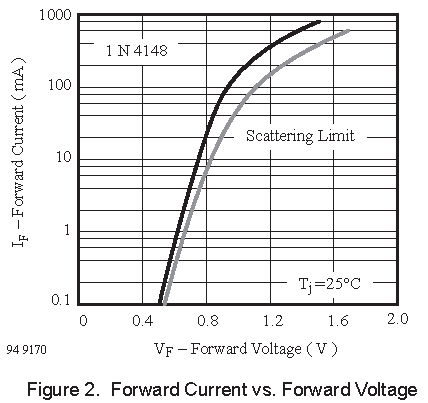
\includegraphics[width=0.5\textwidth]{1N4148}
\end{figure}

\subsection{Solución}

\subsubsection{Equivalente de Thévenin}

$R_t = 10k\Omega || 1650\Omega \approx 1416.31\Omega$

$R_t = 10k\Omega || 1650\Omega \approx 1416.31\Omega$

\begin{align*}
  24300 i_D + v_D &= 10 \cdot 11i_D - 25 \\
  24300 i_D + v_D &= 1650 \cdot 10 i_D\\
  &\Rightarrow i_D = - \frac{25 + v_D}{24289}
\end{align*}

Si $v_D = 0.7V \Rightarrow i_D = $


Circuito en DC:
\begin{figure}[H]
  \begin{center}
    \begin{circuitikz}

      \draw (0, 0)
      to [R, l=$24300\Omega$] (0, 5)
      to [D*, l_=$\mathrm{1N4148}$, i_=$i_D$, v^<=$v_D$] (3, 5)
      to [R, l=$10\Omega$] (3, 2.5)
      to [battery, l=$25V$] (3, 0)
      to [short] (0, 0)
      ;

      \draw (3, 0)
      to [short] (6, 0)
      to [R, l=$1650\Omega$] (6, 5)
      to [american controlled current source, l_=$10i_D$] (3, 5)
      ;

    \end{circuitikz}
  \end{center}
\end{figure}


\section{}

Encuentre los valores mínimo y máximo de $r_i$, si $V_i$ varía entre $80V$ y
$100V$.

\begin{figure}[H]
  \begin{center}
    \begin{circuitikz}

      \draw (0,0)
      to [sV, l=$V_i$] (0, 4)
      to [R, l=$r_i$] (3, 4)
      to [short] (9, 4)
      to [R, l_=$100\Omega$] (9, 0)
      to [short] (0, 0)
      ;

      \draw (3, 0)
      to [zzD*, l=$Z_2$] (3, 2)
      to [zzD*, l=$Z_1$] (3, 4)
      ;

      \draw (3, 2) to [short] (6, 2)
      ;

      \draw (6, 0)
      to [R, l=$430\Omega$] (6, 2)
      to [R, l=$200\Omega$] (6, 4)
      ;

    \end{circuitikz}
  \end{center}
\end{figure}

\begin{align*}
  Z_1 &: \mathrm{1N4740A} \\
  Z_2 &: \mathrm{1N4733A}
\end{align*}

\begin{center}
    \begin{tabular}{ | c | c c c c | c c c | c c c | c | c | }
      \hline
      \multirow{2}{*}{Device} &
      $V_Z$ & $Z_Z$ & \multirow{2}{*}{@} & $I_{ZT}$ &
      $Z_{ZK}$ & \multirow{2}{*}{@} & $I_{ZK}$ &
      $V_R$ & \multirow{2}{*}{@} & $I_R$ &
      $I_{\mathrm{SURGE}}$ &
      $I_{\mathrm{ZM}}$
      \\
      &
      ($V$) & ($\Omega$) & & ($mA$) &
      ($\Omega$) & & ($mA$) &
      ($V$) & & ($\mu A$) &
      ($mA$) &
      ($mA$)
      \\
      \hline
      1N4733A &
      5.1 & 7.0 & \multirow{2}{*}{.} & 49 &
      550 & \multirow{2}{*}{.} & 1.0 &
      1.0 & \multirow{2}{*}{.} & 10 &
      890 &
      178
      \\
      1N4740A &
      10 & 7.0 & & 25 &
      700 & & 0.25 &
      7.6 & & 10 &
      454 &
      91
      \\
      \hline
    \end{tabular}
\end{center}

\subsection{Solución}

\subsubsection{Ecuaciones e Información de los Diodos Zener}

\begin{align*}
  Z_1 :& I_Z = Z_Z V_Z + I_{ZT} - Z_Z V_{Z_T}\\
      & I_Z = \frac{V_Z}{7} - 1.40357 & 0.00025 < I_Z < 0.091\\
      & V_Z = 7 I_Z + 9.825 & 9.827 < V_Z < 10.462\\
  Z_2 :& I_Z = \frac{V_Z}{Z_Z} + I_{ZT} - \frac{V_Z}{Z_Z} \\
       & I_Z = \frac{V_Z}{7} - 0.67957 & 0.001 < I_Z < 0.178 \\
       & V_Z = 7 I_Z + 4.757 & 4.764 < V_Z < 6.003\\
\end{align*}

\subsubsection{Ecuaciones del Circuito}

\begin{equation} \label{eq:zen1}
  \frac{V_i - (V_{Z1}+V_{Z2})}{r_i} = I_{100\Omega} + I_{200\Omega} + I_{Z1}
\end{equation}

\begin{equation*}
  I_{Z1} + I_{200\Omega} = I_{Z2} + I_{430\Omega}
\end{equation*}
\begin{equation} \label{eq:zen2}
  \Rightarrow I_{Z1} = -I_{200\Omega} + I_{Z2} + I_{430\Omega}
\end{equation}

Usamos \ref{eq:zen2} en \ref{eq:zen1}:

\begin{equation} \label{eq:zen3}
  \frac{V_i - (V_{Z1}+V_{Z2})}{r_i} = I_{100\Omega} + I_{Z2} + I_{430\Omega}\\
\end{equation}

Definimos las corrientes por las resistencias de acuerdo a los voltajes de los
diodos:

\begin{align}
  I_{200\Omega} &= \frac{V_{Z1}}{200} \label{eq:zen4} \\
  I_{430\Omega} &= \frac{V_{Z2}}{430} \label{eq:zen5} \\
  I_{100\Omega} &= \frac{V_{Z1} + V_{Z2}}{100} \label{eq:zen6}
\end{align}

Sustituimos \ref{eq:zen5} y \ref{eq:zen6} en \ref{eq:zen3} para obtener la
ecuación de $r_i$ en terminos de las variables de los diodos.

\begin{align}
  \frac{V_i - (V_{Z1}+V_{Z2})}{r_i} &= \frac{V_{Z1} + V_{Z2}}{100} + I_{Z2} + \frac{V_{Z2}}{430} \nonumber \\
  r_i &= \frac{V_i - (V_{Z1}+V_{Z2})}{\frac{V_{Z1} + V_{Z2}}{100} + I_{Z2} + \frac{V_{Z2}}{430}} \label{eq:zen7}
\end{align}

Caso $r_{i_{\mathrm{MAX}}}$\\
$V_{i_{\mathrm{MAX}}}$\\
$I_{Z1} > I_{Z2_{\mathrm{MIN}}} + \frac{V_{Z2_{\mathrm{MIN}}}}{430} = 0.001 + \frac{4.764}{430} \approx 0.012$\\
$V_{Z1}(0.001 + \frac{4.764}{430}) \approx 9.910$\\
$I_{Z2_{\mathrm{MIN}}}$\\
$V_{Z2_{\mathrm{MIN}}}$


Se usan estos valores en \ref{eq:zen7}:\\
$r_i = \frac{100 - (9.910+4.764)}{\frac{9.910+4.764}{100} + 0.001 + \frac{4.764}{430}} \approx 537.25\Omega$

\bigskip

Caso $r_{i_{\mathrm{MIN}}}$\\
$V_{i_{\mathrm{MIN}}}$\\
$I_{Z1_{\mathrm{MAX}}}$\\
$V_{Z1_{\mathrm{MAX}}}$\\
$I_{Z2_{\mathrm{MAX}}}$\\
$V_{Z2_{\mathrm{MAX}}}$

Se usan estos valores en \ref{eq:zen7}:\\
$r_i = \frac{80 - (10.462+6.003)}{\frac{10.462+6.003}{100} + 0.178 + \frac{6.003}{430}} \approx 178.16\Omega$

\section{}

Para la siguiente figura, suponga que los diodos son ideales. Demuestre que los
tres diodos no pueden conducir a la vez. ($V_i$ varia entre 0 y 50 voltios).

\begin{figure}[H]
  \begin{center}
    \begin{circuitikz}

      \draw (0,0)
      to [sV, l=$V_i$] (0, 6)
      to [D*, l=$D_3$] (3, 6)
      to [short] (12, 6)
      to [open, o-o, v^<=$V_o$] (12, 0)
      to [short] (0, 0)
      ;

      \draw (3, 0)
      to [battery, l_=$6V$] (3, 2)
      to [R, l_=$5k\Omega$] (3, 4)
      to [D*, l_=$D_1$] (3, 6)
      ;

      \draw (6, 0)
      to [battery, l_=$20V$] (6, 2)
      to [R, l_=$10k\Omega$] (6, 4)
      ;
      \draw (6, 6) to [D*, l=$D_2$] (6, 4)
      ;

      \draw (9, 0) to [R, l_=$5k\Omega$] (9, 6)
      ;

    \end{circuitikz}
  \end{center}
\end{figure}

\subsection{Solución}

Se formulan las ecuaciones para $V_o$.

\begin{align*}
  V_o &= V_i - V_{D3} \\
  V_o &= 6V - 5k\Omega \cdot I_{D1} - V_{D1} \\
  V_o &= 20V + 10k\Omega \cdot I_{D2} + V_{D2} \\
  V_o &= 5k\Omega \cdot \left( I_{D1} - I_{D2} + I_{D3} \right)
\end{align*}

Se encienden todos los diodos, entonces tenemos que:

\begin{align*}
  V_{D1} &= 0 & V_{D2} &= 0 & V_{D3} &= 0
\end{align*}
\begin{align*}
  I_{D1} &> 0 & I_{D2} &> 0 & I_{D3} &> 0
\end{align*}

Se reformulan las ecuaciones:

\begin{align*}
  V_o &= V_i \\
  V_o &= 6V - 5k\Omega \cdot I_{D1} \\
  V_o &= 20V + 10k\Omega \cdot I_{D2} \\
  V_o &= 5k\Omega \cdot \left( I_{D1} - I_{D2} + I_{D3} \right)
\end{align*}

Se resuelve para $I_{D1}$ y se aplica $I_{D1} > 0$:

\begin{align*}
  V_o = V_i &= 6V - 5k\Omega \cdot I_{D1} \\
  I_{D1} &= \frac{6 - V_i}{5k\Omega} > 0 \\
  & 6V > V_i
\end{align*}

Se resuelve para $I_{D2}$ y se aplica $I_{D2} > 0$:

\begin{align*}
  V_o = V_i &= 20V + 10k \cdot I_{D2} \\
  I_{D2} &= \frac{V_i - 20}{10k\Omega} > 0 \\
  & V_i > 20V
\end{align*}

No se puede dar simultáneamente que $6V > V_i$ y que  $V_i > 20V$, por lo que el
caso en que los 3 diodos estén encendidos no existe.

\end{document}
